\documentclass[]{article}
\usepackage{lmodern}
\usepackage{amssymb,amsmath}
\usepackage{ifxetex,ifluatex}
\usepackage{fixltx2e} % provides \textsubscript
\ifnum 0\ifxetex 1\fi\ifluatex 1\fi=0 % if pdftex
  \usepackage[T1]{fontenc}
  \usepackage[utf8]{inputenc}
\else % if luatex or xelatex
  \ifxetex
    \usepackage{mathspec}
    \usepackage{xltxtra,xunicode}
  \else
    \usepackage{fontspec}
  \fi
  \defaultfontfeatures{Mapping=tex-text,Scale=MatchLowercase}
  \newcommand{\euro}{€}
\fi
% use upquote if available, for straight quotes in verbatim environments
\IfFileExists{upquote.sty}{\usepackage{upquote}}{}
% use microtype if available
\IfFileExists{microtype.sty}{\usepackage{microtype}}{}
\usepackage{longtable,booktabs}
\usepackage{graphicx}
\makeatletter
\def\maxwidth{\ifdim\Gin@nat@width>\linewidth\linewidth\else\Gin@nat@width\fi}
\def\maxheight{\ifdim\Gin@nat@height>\textheight\textheight\else\Gin@nat@height\fi}
\makeatother
% Scale images if necessary, so that they will not overflow the page
% margins by default, and it is still possible to overwrite the defaults
% using explicit options in \includegraphics[width, height, ...]{}
\setkeys{Gin}{width=\maxwidth,height=\maxheight,keepaspectratio}
\ifxetex
  \usepackage[setpagesize=false, % page size defined by xetex
              unicode=false, % unicode breaks when used with xetex
              xetex]{hyperref}
\else
  \usepackage[unicode=true]{hyperref}
\fi
\hypersetup{breaklinks=true,
            bookmarks=true,
            pdfauthor={},
            pdftitle={},
            colorlinks=true,
            citecolor=blue,
            urlcolor=blue,
            linkcolor=magenta,
            pdfborder={0 0 0}}
\urlstyle{same}  % don't use monospace font for urls
\setlength{\parindent}{0pt}
\setlength{\parskip}{6pt plus 2pt minus 1pt}
\setlength{\emergencystretch}{3em}  % prevent overfull lines
\setcounter{secnumdepth}{5}


\begin{document}

%  Titelblad

% Opmerking: gaat uit van een \baselinestretch waarde van 1.5 (die moet
% ingesteld worden voor het begin van de document endvironment)

\begin{titlepage}

\setlength{\hoffset}{-0.3in}
\setlength{\voffset}{-1in}
\setlength{\topmargin}{1.5cm}
\setlength{\headheight}{0.5cm}
\setlength{\headsep}{1cm}
\setlength{\oddsidemargin}{3cm}
\setlength{\evensidemargin}{3cm}
\setlength{\footskip}{1.5cm}
\enlargethispage{1cm}
% \textwidth en \textheight hier aanpassen blijkt niet te werken

\fontsize{12pt}{14pt}
\selectfont

\begin{center}


\includegraphics[height=2cm]{logo.png}

\vspace{0.5cm}

Universidad Sim\'on Bol\'ivar\\
Departamento de computaci\'on\\
Miniproyecto de Desarrollo de Software EP4793\\

\vspace{3.5cm}

\fontseries{bx}
\fontsize{17.28pt}{21pt}
\selectfont

Desarrollo de sistema de permisos \\
para la Coordinación de Computación y\\
procesador de horarios

\fontseries{m}
\fontsize{12pt}{14pt}
\selectfont

\vspace{.6cm}



\vspace{.4cm}


\vspace{3cm}

Tutores : \\
Eduardo Blanco\\
Carolina Mart\'inez\\
\vspace{1cm}
Alumnos: \\
Daniel  Leones \\
Javier  L\'opez \\
Carlos Mart\'inez\\


\vspace{1cm}

1ro de junio del 2016

\end{center}
\end{titlepage}

{
\hypersetup{linkcolor=black}
\setcounter{tocdepth}{3}
\tableofcontents
}
\newpage

\section{Introducción}\label{introducciuxf3n}

(Dejar para el final) Desde que comenzó el auge y la masificación de la
informática los sistemas de información han cumplido un papel
fundamental para reemplazar los métodos manuales de procesar datos,
disminuyendo de esta manera el uso de materiales físicos y horas de
trabajo considerablemente.

En el caso de la Universidad Simón Bolívar, a pesar de que existan
avances en el uso de la tecnología en bastantes áreas administrativas,
aún es posible encontrarse con espacios donde los protocolos se llevan
de manera manual, ocasionando una serie de inconvenientes que sumados a
la crisis universitaria por la cual la Universidad Simón Bolívar está
pasando pueden ser realmente perjudiciales.

Hoy en día existe una gran cantidad de herramientas útiles y de acceso
libre que sirven para desarrollar software utilizando tan solo un
computador personal y conocimientos adquiridos durante la carrera de
Ingeniería de la Computación, de manera considerablemente rápida y lo
suficientemente poderosa para el problema a resolver.

Este informe tiene como objeto servir de explicación de como utilizando
algunas de estas herramientas fue resuelto un problema de ineficiencia
burocrática de tiempo y recursos mediante la aplicación de conocimientos
del área de la computación como parte de un Miniproyecto de Desarrollo
de Software.

\section{Resumen}\label{resumen}

(Dejar para el final) Durante el desarrollo del presente se explicarán a
detalle puntos esenciales para entender el trabajo ejecutado y el
objetivo del mismo.

Se comenzará planteando el problema, explicando la situación de la
coordinación de Ingeniería de la Computación donde el procesamiento de
permisos funciona de manera manual, haciendo uso de una planilla donde
los estudiantes llenan un formulario solicitando su permiso, lo cual
requiere un uso considerable de papel y tinta para imprimir además de
ser un problema de personal para la coordinación ya que la coordinadora
debe procesar manualmente cada permiso y revisar el expediente de cada
estudiante solicitante, tomar la decisión que se considere apropiada y
luego escribir manualmente los archivos de tipo CSV en el formato que
recibe DACE. En esta sección también es mencionada.

Luego de esto, se mencionan los objetivos del Miniproyecto, sección
donde se explica la manera en la que se resolverá el problema planteado
una vez culminado el Miniproyecto. En esta sección son explicados los
módulos del programa donde se le provee a los distintos actores que
interactuarán con el sistema interfaces para realizar sus funciones
correspondidas así como también los módulos que realizan de manera
automatizada procesos que solían ser manuales.

Después comienza la parte de análisis, donde se explica de una manera
menos general y más técnica la lógica de programación del sistema así
como también el detalle de la arquitectura utilizada en el mismo, tales
como la explicación de cada módulo y el lenguaje de programación junto a
todas las librerías utilizadas en el desarrollo.

Por último, en el informe se habla del plan de pruebas y los resultados.
En esta parte se explica el procedimiento utilizado para probar cada
módulo del sistema, conseguir errores y repararlos de manera segura.
También se mencionan los resultados obtenidos una vez realizada la
prueba y procesados los permisos.

\section{Planteamiento del problema}\label{planteamiento-del-problema}

La Coordinación de Ingeniería de Computación trimestralmente y como
parte de sus funciones debe controlar los permisos de inscripción de los
estudiantes adscritos a esta carrera, en los cuales se contempla la
inscripción de materias electivas, límite de créditos (superiores e
inferiores a la norma), materias cuyos requisitos no han sido cubiertos
totalmente y materias fuera del plan de estudio por nombrar algunos.

Para que los estudiantes de Ingeniería de Computación pudieran solicitar
sus permisos debían llenar planillas que la coordinación proporcionaba,
en donde era necesario escribir los permisos requeridos y marcar en un
grafo (que representa el pensum de la carrera) las materias aprobadas,
las cursadas en el trimestre actual y las que se desean inscribir.

La coordinación, para que los estudiantes realizaran este proceso debía
imprimir planillas de permisos para cada uno, recibirlas después de
llenadas y resolver las posibles inquietudes de cada estudiante.
Posteriormente para procesar cada permiso, la coordinadora debía
descargar todos los expendientes de los estudiantes para comprobar que
los grafos llenados por ellos coincidieran con los datos oficiales de la
universidad. Luego, tomando en cuenta el índice de los estudiantes, su
situación y la cantidad de cupos disponibles para cada asignatura
procedía a aprobar o negar los diferentes permisos soliticitados.

Adicionalmente a esto, es necesario enviar correos a cada una de los
estudiantes cuyas solicitudes de permiso han sido negadas para que
reconsideren su plan de inscripción. La generación de cada uno de estos
correos personalizados se realizaba uno a uno manualmente.

Por último, la coordinación con los datos de los permisos aprobados,
generaba de forma manual tres hojas de cálculo para DACE: uno para los
permisos de asignaturas, un memo con los permisos de generales y un
tercer archivo con datos con permisos generales y de límites de
créditos.

Para los permisos del trimestre enero-marzo 2017, hubiese sido necesario
procesar de forma manual los permisos de más de 140 estudiantes, lo cual
representa, aproximadamente 400 permisos diferentes. La única etapa en
el procesamiento de permisos apoyada por software adaptado a las
necesidades de la coordinación era la visualización del grafo de los
estudiantes, el cual es uno de los módulos realizados como parte de un
miniproyecto anterior.

El miniproyecto precedente consistía en una aplicación móvil la cual
requería un servidor para atender las solicitudes de todos los
estudiantes y una aplicación de escritorio para el procesamiento de
estos. Los inconvenientes encontrados con el uso de esta aplicación
radicaban en: la ausencia de un servidor para el alojamiento de la
aplicación, la ausencia de un módulo para descargar los expendientes de
los estudiantes y fallas en el cumplimiento de los requerimientos de
coordinación (todos los permisos de un estudiante eran tomados como una
unidad monolítica en vez de elementos individuales).

\section{Objetivos del miniproyecto}\label{objetivos-del-miniproyecto}

El objetivo de este Miniproyecto de Desarrollo de Software es
implementar un sistema capaz de proveerle a los estudiantes de
Ingeniería de la Computación de la Universidad Simón Bolívar una
herramienta para solicitar los permisos relacionados con la inscripción
de materias de una manera más fácil y cómoda de utilizar y a su vez
mucho más barata y ecológica ya que como se mencionó en el punto
anterior, quedaría eliminado el uso innecesario de papel y tinta de
impresiones para la solicitud de estos permisos.

A su vez, del lado del procesamiento de los permisos, es objetivo del
Miniproyecto proveerle a la coordinadora de la carrera un programa con
interfaz sencilla, efectiva y poderosa para el procesamiento manual de
los permisos solicitados por los estudiantes. La herramienta provista
deberá ser capaz de descargar los permisos, almacenarlos, descargar los
respectivos expedientes académicos de manera automática, llevar control
de su estado de aprobación y una vez finalizado todo el procesamiento,
debe poder notificar a los estudiantes el estado de sus permisos y
generar archivos en formatos específicos para la Dirección de Adimisión
y Control de Estudios (DACE)

Todo lo mencionado logrará cumplir con el objetivo general de este
Miniproyecto de automatizar una serie de tareas que hasta este trimestre
han sido manuales y ahorrar una cantidad considerable de tiempo,
esfuerzo y dinero a la coordinación de Ingeniería de la Computación.

\section{Análisis}\label{anuxe1lisis}

Para entender mejor el sistema presentamos paso a paso el proceso que
realiza la coordinación para poder dar respuesta a las solicitudes de
permioso, primero se presentará el algoritmo de trabajo seguido y
posteriormente las reglas necesarias para el cumplimiento de los
objetivos iniciales del miniproyecto.

\subsection{Flujo de trabajo posterior a la
implemenación}\label{flujo-de-trabajo-posterior-a-la-implemenaciuxf3n}

Luego de la implemenación del sistema procesador de permisos, la
coordinación para poder procesar los permisos debe publicar el link al
formulario de permisos y activarlo para aceptar las respuestas de los
estudiantes, al terminar el período de soliticiud se desactiva el
formulario y se inicia el procesamiento.

Antes procesar todas las respuestas estudiantes la coordinadora deberá
utilizar el módulo de \emph{descargar permisos} (ver figura 1
\ref{fig1}), el cual descargará la hoja de cálculo (alojada en Google
Drive), adicionalmente a esto se descargarán los expedientes académicos
de todos los estudiantes presentes en la solicitud y se generarán de
forma automática los flujográmas respectivos representando las materias
ya cursadas

\begin{figure}[htbp]
\centering
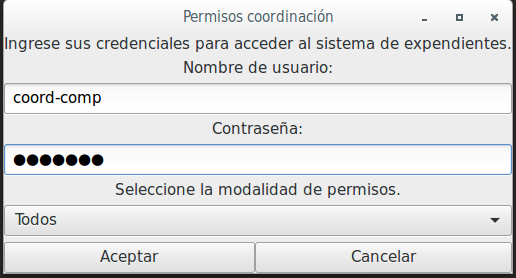
\includegraphics{descarga.png}
\caption{figura 1 - Vista de descarga de permisos \{fig1\}}
\end{figure}

Posteriormente la coordinación puede aprobar y negar permisos, para ello
se debe utilizar el módulo \emph{programa de permisos} en donde se
pueden realizar diferentes consultas sobre los estudiantes, buscar
permisos por materia, por tipo de permiso y por estado (ver figura 2
\ref{fig2}). También se requiere hacer un análisis

\begin{figure}[htbp]
\centering
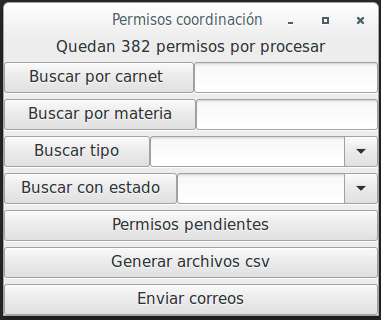
\includegraphics{principal.png}
\caption{figura 2 - Menu principal \{fig2\}}
\end{figure}

Por último con los módulos de \emph{enviar correos} (figura 3 \ref{fig3}
y 4 \ref{fig4}) y \emph{generar archivos csv} se envían las
notificaciones a cada estudiante si sus permisos fueron negados y se
generan las tablas para DACE en formato CSV (Comma-Separated Values).
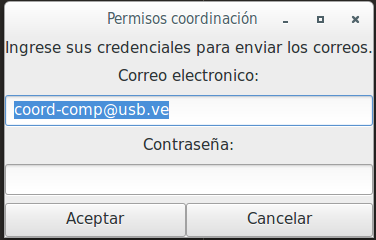
\includegraphics{correos.png} 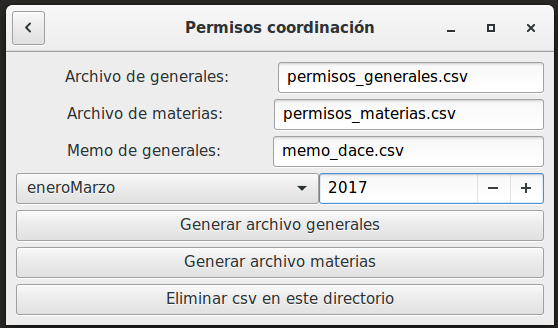
\includegraphics{csv.png}

Antes de iniciar un nuevo proceso de recepción de permisos se debe
limpiar la hoja de cálculo de Google Drive y la base de datos de la
aplicación de escritorio.

De forma resumida el flujo para el procesamiento de permisos se realiza
en los siguientes pasos:

\begin{enumerate}
\def\labelenumi{\arabic{enumi}.}
\itemsep1pt\parskip0pt\parsep0pt
\item
  Limpiar hoja de cálculo y base de datos, activar y publicar el
  formulario
\item
  Descargar permisos de estudiantes
\item
  Aprobar y negar permisos
\item
  Enviar correos y tablas de resultados
\end{enumerate}

De forma gráfica la figura 5 representa los pasos a tomar, en donde los
bloques coloreados son las acciones ya automatizadas y las restantes las
cuales solo pueden ser realizadas de forma manual.

\begin{figure}[htbp]
\centering
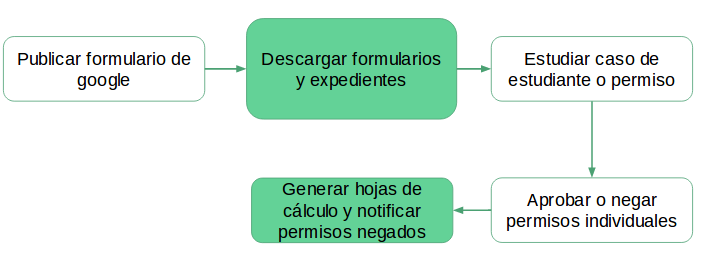
\includegraphics{flujo.png}
\caption{figura 5 - Flujo de trabajo \{fig5\}}
\end{figure}

\subsection{Especificación de reglas}\label{especificaciuxf3n-de-reglas}

Las reglas de trabajo pueden ser especificadas en los siguientes 4
conjuntos:

\begin{itemize}
\itemsep1pt\parskip0pt\parsep0pt
\item
  Restricciones de formulario y permisos
\item
  Visualización de datos en pantalla
\item
  Formato de tablas para dace
\item
  Especificación de correos
\end{itemize}

Las restricciones se relacionan directamente con diferentes aspectos
como la base de datos, la interfaz gráfica, las reglas de trabajo que
son parte del procesamiento de los permisos y el~formato de salida del
programa. A continuación serán presentadas las reglas de cada uno de
estos conjuntos.

\subsubsection{Restricciones de
formulario}\label{restricciones-de-formulario}

Antes de seleccionar Google Form como herramienta para almacenar las
solicitudes se tuvo que verificar que la~plataforma tuviese soporte para
la verificación de credenciales institucionales y lo cumplió,
adicionalmente fue elegida ya que se tenían restricciones en cuanto al
uso de servidores para alojar una aplicación web propia y esta solución
ya se había intentando en el miniproyecto anterior sin éxito.

Al diseñar el formulario que los estudiantes llenarían se tomó en cuenta
el formato ya existente para poder cubrir de manera completa todos los
tipos de permisos necesarios, también fue necesario realizar
verificaciones de campos mediante expresiones regulares, rangos
numéricos y de opciones de permisos que eran mutuamente excluyentes.

\subsubsection{Visualización de datos en
pantalla}\label{visualizaciuxf3n-de-datos-en-pantalla}

Los requerimientos de la interfaz incluían las siguientes reglas
puntuales:

\begin{itemize}
\itemsep1pt\parskip0pt\parsep0pt
\item
  Poder observar los grafos con materias aprobadas.
\item
  Permitir la consulta todos los permisos pendientes y tenerlos de forma
  adyacente para poder procesarlos de manera rápida.
\item
  Visualización de todos los permisos de un tipo específico.
\item
  Consulta para los permisos de materias electivas y visualización de la
  cantidad de permisos ya aprobados y pendientes para poder decidir a
  que estudiantes otorgar los puestos disponibles (los cuales son
  limitados)
\item
  Que permitiera observar todos los permisos de un estudiante para poder
  estudiar mejor su situación académica y para decidir con base en su
  conjunto de datos (índice, créditos aprobados, materias aprobadas).
\item
  Visualización de los datos personales de los estudiantes para poder
  tener comunicación si es necesario (correos, número de teléfono y
  nombre)
\end{itemize}

Todas estas reglas fueron seguidas en la implemenación del sistema.

\subsubsection{Formato de tablas}\label{formato-de-tablas}

Las tablas generadas debían estar en formato xls o xlsx, o cualquier
otro que pudiese ser importado por Libre Office y pudiese ser exportado
a un archivo con alguna de las extensiones ya mencionadas.

En cuanto a las reglas de generación de las tablas, cada uno de los tres
archivos requeridos por DACE requiere un orden de las columnas como se
puede observar a continuación en formato CSV:

\begin{itemize}
\item
  Para el archivo de materias

\begin{verbatim}
COD_ASIGNATURA,ANIO_CARNET,NUM_CARNET,SIGLO,ANIOP,MESIP,
MESFP,BLOQUE,SECCION,NRO_CREDITOS,PERMISO,RENGLON,
NOTA_ASIGNATURA,IND_NOTA_SIN_EFECTO
\end{verbatim}
\item
  Para el archvivo de permiso generales

\begin{verbatim}
ANIO_CARNET,NUM_CARNET,SIGLO,ANIOP,MESIP,MESFP,SITUACION,
SITUACIONINSCRIP,GENERAL,LIMITE CR,
=NOTA_X_CREDITO_PONDERADO,TOTAL_CREDITOS,PP
\end{verbatim}
\item
  Para el memo

\begin{verbatim}
N°,CARNÉ,NOMBRES Y APELLIDOS.,PERMISO,PERIODO
\end{verbatim}
\end{itemize}

Cada permiso aprobado puede aparecer en uno o varios de estos archivos
dependiendo de su tipo, para los dos primeros archivos mencionados
existen algunos parámetros fijos como \emph{``SIGLO''} el cual siempre
posee un valor de \emph{`1'} y \emph{``PERMISO''} en donde vale
\emph{`s'} (ya que el archivo solo posee permisos aprobados).

Las columnas de \emph{``ANIO\_CARNET''} y \emph{``NUM\_CARNET''} poseen
el carnet del estudiante separando el año de la cohorte del resto del
número de 7 dígitos, las columnas \emph{``ANIOP''}, \emph{``MESIP''} y
\emph{``MESFP''} especifican el período para el cual será vaĺido el
permiso mediante año, número de mes del inicio del trimestre y número
del mes de finalización respectivamente.

Por último para cada tipo de permiso se deben generar las siguientes
salidas en cada unos de los archivos:

\begin{itemize}
\itemsep1pt\parskip0pt\parsep0pt
\item
  PP: Agregar créditos en archivo de materias
\item
  Dos Generales: Agregar E2 en la columna ``GENERAL'' del archivo de
  generales y agrega en memo.
\item
  Límite de créditos: agregar número de créditos en columna ``LIMITE
  CR'' del archivo de generales.
\item
  Permiso de electiva: agregar código en columna ``COD\_ASIGNATURA'' del
  archivo de materias.
\item
  Sin requisito: agregar código de la asignatura en la columna
  ``COD\_ASIGNATURA'' del archivo de materias.
\item
  Se debe agregar el código de asignatura en ``COD\_ASIGNATURA'' del
  archivo de materias y una línea el en archivo de memos para los
  siguientes tipos:

  \begin{itemize}
  \itemsep1pt\parskip0pt\parsep0pt
  \item
    General extra
  \item
    Extraplan
  \item
    Extraplan de general más un general
  \item
    Extraplan de general
  \end{itemize}
\end{itemize}

\subsubsection{Especificación de
correos}\label{especificaciuxf3n-de-correos}

Para en el envío de correos se especificó que solo se enviaran correos a
cada uno de estudiantes con permisos negados, debía ser un mensaje único
especificando todos los permisos negados.

\section{Diseño}\label{diseuxf1o}

La aplicación se encuentra distribuida en los siguientes módulos y
plataformas:

\begin{itemize}
\itemsep1pt\parskip0pt\parsep0pt
\item
  Plataforma google: a través de google form los usuarios realizan sus
  solicitudes de permisos, estos resultados son almacenados en una hoja
  de cálculo disponible en google drive para ser procesada
  posteriormente por la aplicación de escritorio.
\item
  Generador de grafos: módulo del miniproyecto anterior, genera archivos
  png con los grafos coloreados con las materias aprobadas de un
  estudiante cualquier en computación.
\item
  Módulo de extración de expedientes: automatiza la búsqueda de
  expedientes mediante las credenciales de la coordinadora de
  computación, realiza consultas en la página
  {[}http://expediente.dii.usb.ve/{]} http://expediente.dii.usb.ve/ y
  almacena los archivos en formato html.
\item
  Módulo csv: permite la generación de tablas en formato csv, requerido
  por dace, es el producto resultante del procesamiento de todos los
  permisos.
\item
  Módulo de bd: mantiene en disco los datos de todos los estudiantes que
  se encuentran solicitando permisos, los tipos de permisos que
  requieren y el estado en el que se encuentran (aprobados, negados o
  pendientes).
\item
  Módulo consulta de formulario: integra las hojas de cálculo de la
  plataforma de google, el de extracción de expedientes, generación de
  grafos y el manejador de base de datos.
\item
  Aplicación de escritorio: unifica todos los módulos ya mencionados
  empleando una interfaz gráfica intuitiva para ser manejada por la
  coordinadora de computación.
\end{itemize}

Para el módulo de procesamiento de formularios y expedientes seguimos el
siguiente algoritmo

\begin{verbatim}
proc procesar_formulario(form):
    por cada fila en form:
        obtener_expediente(fila['carnet'])
        generar_grafo(archivo_carnet,fila[carnet])
        insertar_en_bd(fila['datos_de_estudiante'])

        por cada permiso en fila:
            insertart_en_bd(permiso)
\end{verbatim}

El diseño de las vistas para la aplicación de escritorio se realizó
mediante la extensión de clases proporcionadas por Gtk para python.
(CAMBIAR O ELIMINAR)

La correspondencia entre el diseño y la implementación programática del
sistema se asocia de la manera expuesta en la siguiente tabla

\newpage

\begin{longtable}[c]{@{}ll@{}}
\toprule\addlinespace
Módulo de diseño & Clase en la implementación
\\\addlinespace
\midrule\endhead
Plataforma google & Implementado directamente
\\\addlinespace
& con la herramienta de Google
\\\addlinespace
Generador de grafos & createPngGraph.class
\\\addlinespace
Módulo de extración de expedientes & coord\_crawler.py
\\\addlinespace
Módulo csv & csv\_creator.py
\\\addlinespace
Módulo de bd & perm\_store.py
\\\addlinespace
Módulo consulta de formulario & check\_answers.py
\\\addlinespace
Aplicación de escritorio & main\_app.py
\\\addlinespace
\bottomrule
\end{longtable}

\subsection{Arquitectura}\label{arquitectura}

Este miniproyecto fue desarrollado en \emph{python3}, haciendo uso de
las siguiente bibliotecas disponibles a través del manejador de paquete
\emph{pip}:

\begin{itemize}
\itemsep1pt\parskip0pt\parsep0pt
\item
  gspread: utilizado para realizar consultas a las hojas de cálculo
  almacenadas en google drive.
\item
  oauth2client: necesario para el proceso de autenticación de google
  drive.
\item
  selenium: biblioteca para realizar automatizaciones sobre exploradores
  web, adicionalmente hacemos uso de chromium webdriver de 64 bits para
  mantener el explorador web en un entorno aislado e indpendente del
  administrador de paquetes del sistema operativo. {[}1{]}
\item
  gi, gi.repository,Gtk: bibliotecas estándar de python3 (en versiones
  nuevas), permiten crear interfaces de escritorio orientadas a eventos.
\item
  easygui: biblioteca que provee ventanas y pop-ups de interacción
  preelaborados.
\item
  sqlite3: \emph{wrapper} de C en \emph{python3} para el sistema de
  gestión de bases de datos portable \emph{sqlite3}. No requiere ser
  instalada, es parte de python3
\item
  csv: biblioteca estándar de python3 que ayuda a generar archivos csv
  (Comma Separated Values), los cuales pueden ser importados en
  cualquier programa de hojas de cálculo (requerido por DACE).
\item
  bs4: módulo de la biblioteca BeautifulSoup, parser de html, permite la
  extración del nombre, índice y número de créditos aprobados por cada
  estudiante desde su expediente.
\end{itemize}

Este proyecto, adicionalmente hace uso de de la máquina virtual de java
8 para la generación de los grafos de cada estudiante y del selenium
webdriver (el cual es dependiente de la arquitectura x86\_64 pero puede
ser sustuido por x86).

La aplicación de escritorio ya se encuentra operativa en uno de los
equipos de la coordinación.

\subsection{Plan de pruebas y
resultados}\label{plan-de-pruebas-y-resultados}

(Describir el an y resultados de ejecución) Durante el desarrollo del
Miniproyecto constantemente cada módulo fue probado mediante permisos de
prueba creados por los desarrolladores directamente en el formulario de
Google los cuales cumplían la función de asegurar la inexistencia de
errores en el procesamiento para cada tipo de permiso.

Al momento de finalizado el sistema con todos sus módulos listos se
decidió que la mejor manera de realizar la prueba era mediante la
solicitud de permisos formal para el trimestre Enero - Marzo 2017, de
esta manera se propagó por todos los medios al alcance el link hacia el
formulario de Google donde los estudiantes por una semana enviaron sus
solicitudes de permisos que vendrían siendo la primera suite de pruebas
completa para el sistema desarrollado.

Esta decisión para las pruebas se debió a que en caso de cualquier error
estos no iban a significar algún tipo de pérdida de la información
suministrada por los estudiantes asomando la posibilidad de realizar una
segunda jornada de solicitud de permisos, ya que en la arquitectura del
sistema al momento de tratar con la información almacenada en la nube es
únicamente para su lectura. Se descargan los permisos, se almacenan
localmente y luego se realiza cualquier prueba necesaria sobre éstos y
en el peor de los casos sencillamente se vuelven a descargar sin ningún
inconveniente.

Proceso de realización de las pruebas:

\begin{itemize}
\itemsep1pt\parskip0pt\parsep0pt
\item
  Recopilación de 416 permisos solicitados entre 142 estudiantes de
  Ingeniería de la Computación a través del Google Form.
\item
  Pruebas de modificar errores cometidos por los estudiantes al momento
  de solicitar los permisos. Errores leves, reconocibles y fáciles de
  arreglar directamente en la hoja de cálculo en la nube.
\item
  Procesamiento de los permisos.
\item
  Creación de los CSV de salida de 366 permisos correctos procesados.
\item
  Envío de correos anunciando permisos negados.
\end{itemize}

Durante la ejecución de las tareas mencionadas anteriormente se pudo
comprobar la correctitud del sistema salvo por errores leves que fueron
solucionados fácilmente sin exponer la integridad de los datos de los
estudiantes en ningún momento.

Los resultados fueron 366 permisos procesados, 50 permisos incorrectos
por errores de los estudiantes al momento de ingresar y tres archivos de
tipo CSV con los resultados del procesamiento en el formato que recibe
DACE.

Errores típicos de código solían ser de inconsistencia de datos. Por
parte de los solicitantes de permisos solían ser ingreso de texto en
campos de códigos de materias lo cual el sistema reconocía cada palabra
como un código de materia lo cual no es causante de mayores
inconvenientes ya que con ser dejados en modo ``pendiente'' son
ignorados por el sistema al momento de generar la salida en CSV.

\section{Conclusión}\label{conclusiuxf3n}

(Dejar para el final) Uno de los objetivos fundamentales de la carrera
de Ingeniería de la Computación es formar a los estudiantes con
conocimientos útiles para automatizar procesos y reducir el uso tanto de
materiales físicos como de tiempo invertido en horas de trabajo.

Gracias al avance de la tecnología, la masificación de los dispositivos
electrónicos y el acceso a internet, la libre propagación de
conocimiento que se refleja en la gran variedad de herramientas libres
para el uso de cualquiera y los conocimientos adquiridos en la carrera
fue posible mejorar considerablemente el proceso administrativo
realizado cada trimestre consecuente a la solicitud y procesamiento de
los permisos para inscripción de trimestres.

La computación existe para facilitar y volver más eficiente el día a día
de los seres humanos, eliminando problemas, reduciendo tiempos de
esperas, uso de recursos que pudiesen ser costosos o poco ecológicos y
reduciendo uso de energía, de manera que todos estos recursos
mencionados puedan ser utilizados en otras áreas del día a día del
hombre y así poder avanzar individual y colectivamente como humanidad.

\section{Bibliografía}\label{bibliografuxeda}

(Dejar para el final)

{[}1{]}

\end{document}
